\chapter*{About Author}\label{author}

%~ \vspace{-3.8cm}

%~ {\hspace{3.4cm}\Large{About Author}}

\vspace{-.8cm}

\begin{figure}[H]
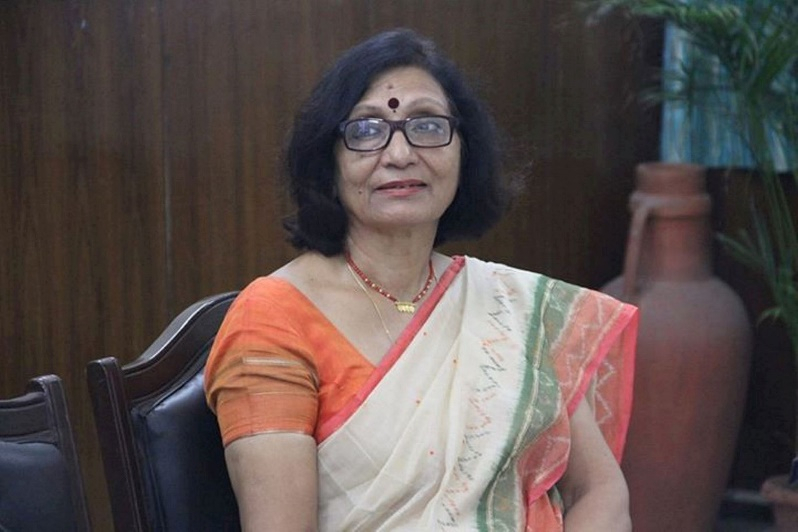
\includegraphics[scale=1]{images/author.jpg}
\caption*{Dr. Vibha Tripathi}
\end{figure}

\vspace{-.5cm}

Dr.~Vibha Tripathi is former Professor and Head Department of Ancient Indian History, Culture \& Archaeology, Banaras Hindu University. She has been Emeritus Professor in the same department. Dr. Tripathi has worked and contributed extensively in the field of Proto-historic and Early Historic Archaeology of India. Professor Tripathi is a keen and versatile scholar and her works reflect a multi- disciplinary approach to study of the past. She emphasizes on holistic reconstruction of the past through her works. Over the last decades, she has conducted excavations at several archaeological sites and published their reports. She has written more than 200 papers and ten books on various aspects of Ancient Indian History, Culture and Archaeology. She has organized number of International and National seminars. Her contributions in the field of ancient Indian technology, especially in ceramics and metallurgy are well known. She was awarded Projects to work on ancient Indian mining and metallurgy by Indian National Science Academy (INSA) and Department of Science and Technology (DST), Government of India. 

She is widely travelled participating and chairing sessions in seminars and symposia in India and abroad.~She has delivered keynote addresses on many such occasions.~She is member of several societies and important national bodies for History of Science, Indian National Science Academy (INSA); Science and   Heritage Research Initiative (SHRI), Department of Science and Technology (DST), Government of India. As a member of such important National and International academic bodies, she continues to contribute to National policies on study of heritage of India. In recognition to her sustained contributions to the field of Ancient Indian Culture and Archaeology, she has received prestigious awards like the ‘Bharatiya Manisha Sutram’ award and V.S. Wakankar Award (2017). More recently, she was awarded Newton Funding by STFC Rutherford Appleton Laboratory, Oxford and Jawaharlal Nehru Centre for Advance Scientific Research to undertake in-depth research in the field of archaeo-metallurgy.

\label{endauthor}
